\chapter{Исследовательская часть}

\section{Технические характеристики}

Технические характеристики устройства, на котором выполнялось тестирование:
\begin{itemize}
	\item операционная система MacOS Monterey 12.3;
	\item 16 ГБ оперативной памяти;
    \item процессор Apple M1~\cite{M1}.
\end{itemize}

Тестирование проводилось на ноутбуке, включенном в сеть электропитания. 
Во время тестирования ноутбук был нагружен только встроенными приложениями окружения, окружением, а также непосредственно системой тестирования.

\section{Постановка исследования}

Целью исследования является нахождение зависимости времени проверки
целостности данных на уровне приложения и базы данных от количества записей в таблице.

Курс может иметь несколько состояний в процессе подготовки материала преподавателем. Черновик курса может редактироваться преподавателем, после чего он должен быть переведен в состояние готовности. Для этого необходимо проверить, что курс удовлетворяет следующим требованиям:
\begin{itemize}
    \item в курсе присутствует один или более теоретический или видео урок;
    \item в курсе присутствует один или более практический урок;
    \item все практический уроки курса должны иметь хотя бы один тест;
    \item максимальная оценка, выставляемая за прохождение урока, всех уроков должна быть больше нуля.
\end{itemize}

Данные проверки целостности курса могут быть проведены как на уровне базы данных, так и на уровне приложения. Необходимо сравнить временные характеристики выполнения для обоих способов. 

Исследование проводится на случайных данных, при этом количество курсов в таблице равно 10, для каждого из которых необходимо провести проверку целостности. Замеры времени проводятся для двух диапазонов данных. Замеряется время проверки целостности курса для количества уроков от 100 до 2000 и от 1000 до 10000. Количество тестов в практических уроках фиксировано и равно 10. Тестовые данные генерируются с помощью библиотеки Faker~\cite{faker}.

\section{Результаты исследования}

В таблице \ref{tbl:time1} приведены результаты замеров времени выполнения реализации проверки целостности курса для количества уроков в курсе от 1000 до 10000 штук.

\begin{table}[H]
    \caption{\label{tbl:time1}Результат замеров времени проверки целостности для количества записей от 1000 до 10000 с шагом 1000.}
	\resizebox{\textwidth}{!}{
	\def\arraystretch{1}
    \begin{tabular}{|r|r|r|}
    \hline
    Количество уроков в курсе, шт &
      \begin{tabular}[c]{@{}r@{}}Время выполнения \\ проверок целостности на \\ уровне приложения, мс\end{tabular} &
      \begin{tabular}[c]{@{}r@{}}Время выполнения \\ проверок целостности на \\ уровне базы данных, мс\end{tabular} \\ \hline
    1000  & 60   & 15   \\ \hline
    2000  & 219  & 85   \\ \hline
    3000  & 616  & 229  \\ \hline
    4000  & 899  & 339  \\ \hline
    5000  & 1102 & 456  \\ \hline
    6000  & 713  & 265  \\ \hline
    7000  & 2457 & 1080 \\ \hline
    8000  & 1603 & 684  \\ \hline
    9000  & 3467 & 1431 \\ \hline
    10000 & 1040 & 437  \\ \hline
    \end{tabular}
    }
\end{table}

\pagebreak
По таблице \ref{tbl:time1} был построен график \ref{img:plot1}. 

\begin{figure}[H]
	\centering
	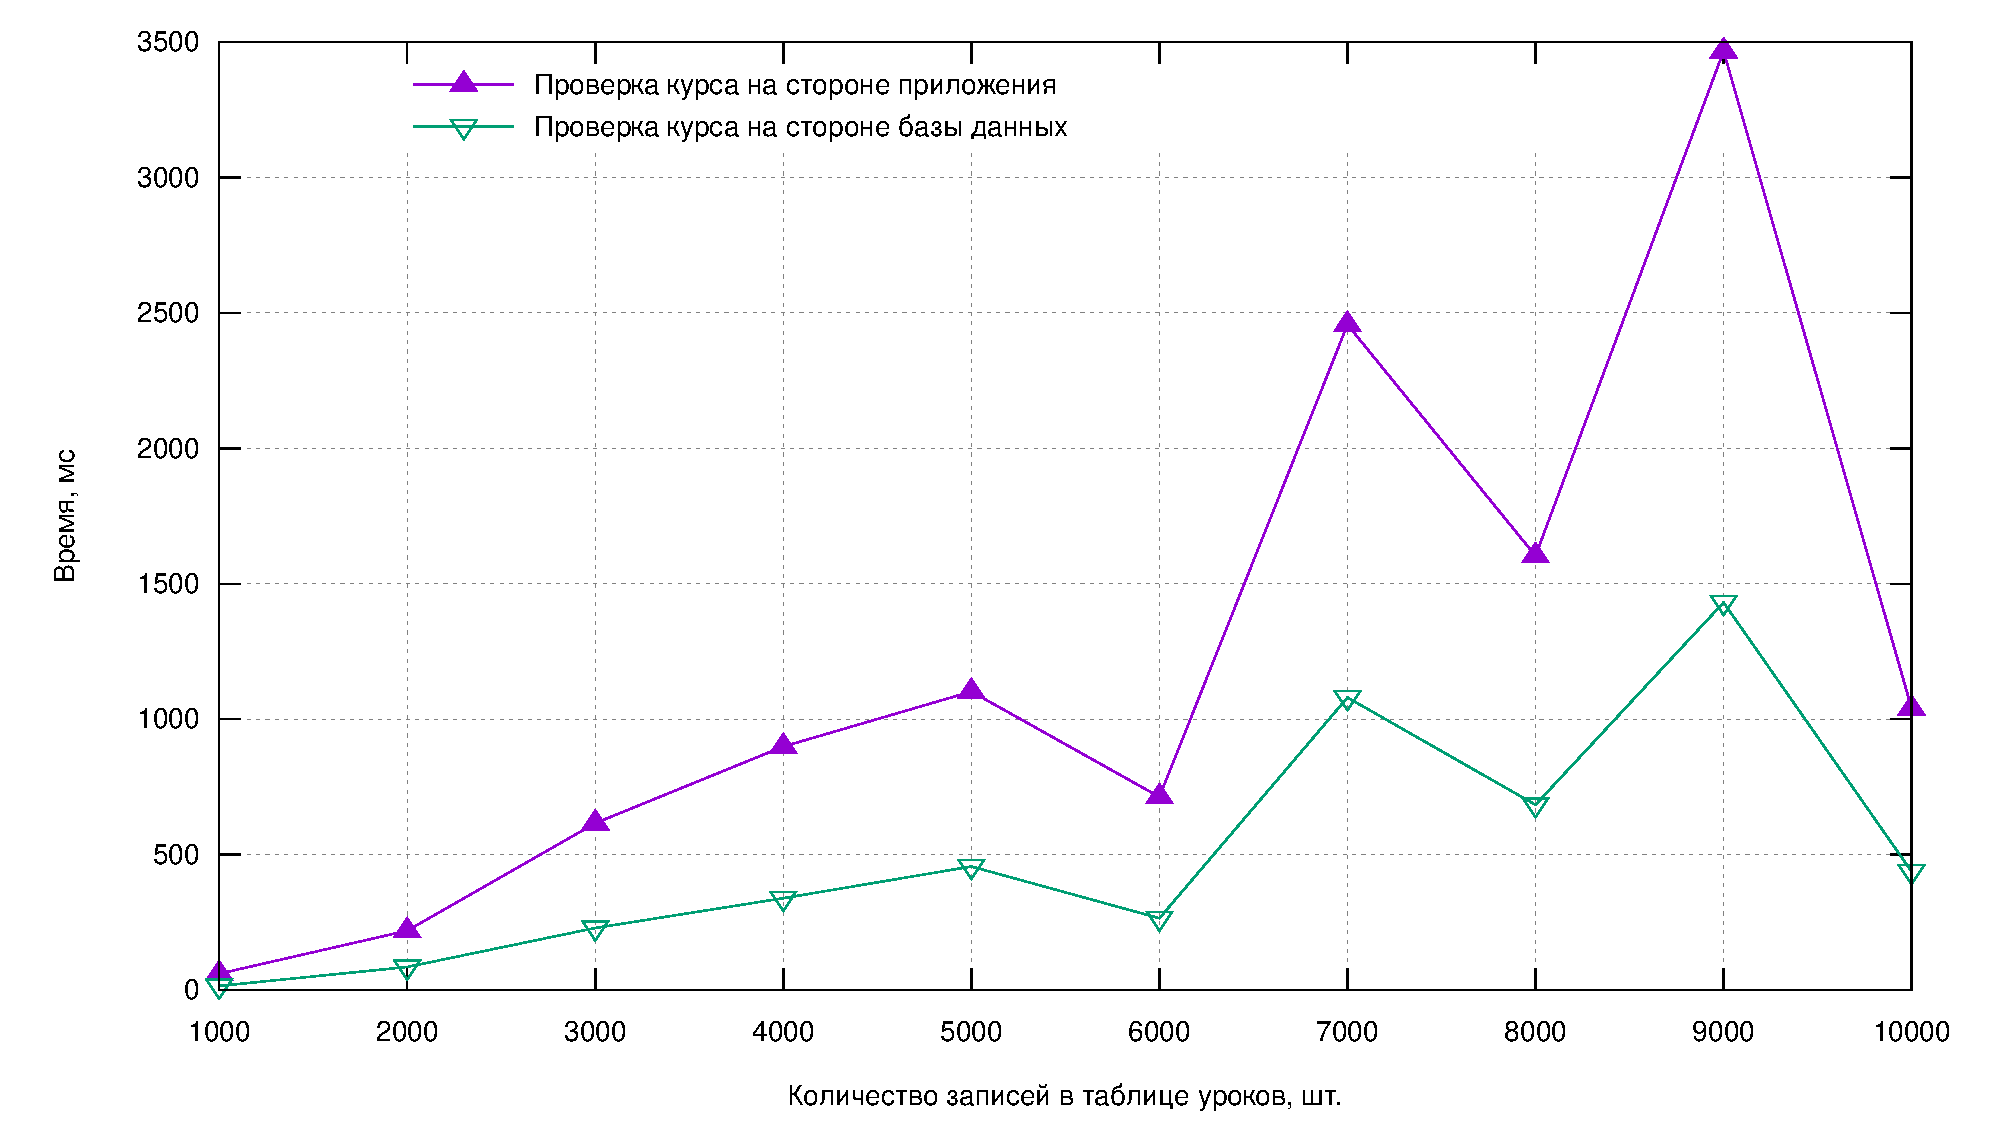
\includegraphics[height=0.35\textheight]{inc/img/plot1.pdf}
	\caption{График зависимости времени проверок целостности от количества уроков в курсе при диапазоне значений от 1000 до 10000}
	\label{img:plot1}
\end{figure}

В таблице \ref{tbl:time2} приведены результаты замеров времени выполнения реализации проверки целостности курса для количества уроков в курсе от 1000 до 10000 штук.

\begin{table}[H]
    \caption{\label{tbl:time2}Результат замеров времени проверки целостности для количества записей от 100 до 2000 с шагом 100.}
	\resizebox{\textwidth}{!}{
	\def\arraystretch{1}
    \begin{tabular}{|r|r|r|}
    \hline
    Количество уроков в курсе, шт &
      \begin{tabular}[c]{@{}r@{}}Время выполнения \\ проверок целостности на \\ уровне приложения, мс\end{tabular} &
      \begin{tabular}[c]{@{}r@{}}Время выполнения \\ проверок целостности на \\ уровне базы данных, мс\end{tabular} \\ \hline
    100  & 24  & 2   \\ \hline
    200  & 12  & 1   \\ \hline
    300  & 13  & 2   \\ \hline
    400  & 24  & 5   \\ \hline
    500  & 37  & 8   \\ \hline
    600  & 47  & 11  \\ \hline
    700  & 52  & 11  \\ \hline
    800  & 27  & 7   \\ \hline
    900  & 48  & 11  \\ \hline
    1000 & 51  & 11  \\ \hline
    1100 & 76  & 22  \\ \hline
    1200 & 107 & 46  \\ \hline
    1300 & 72  & 21  \\ \hline
    1400 & 112 & 37  \\ \hline
    1500 & 100 & 32  \\ \hline
    1600 & 164 & 60  \\ \hline
    1700 & 118 & 40  \\ \hline
    1800 & 287 & 110 \\ \hline
    1900 & 190 & 71  \\ \hline
    2000 & 166 & 61  \\ \hline
    \end{tabular}
    }
\end{table}

\pagebreak
По таблице \ref{tbl:time2} был построен график \ref{img:plot2}. 

\begin{figure}[H]
	\centering
	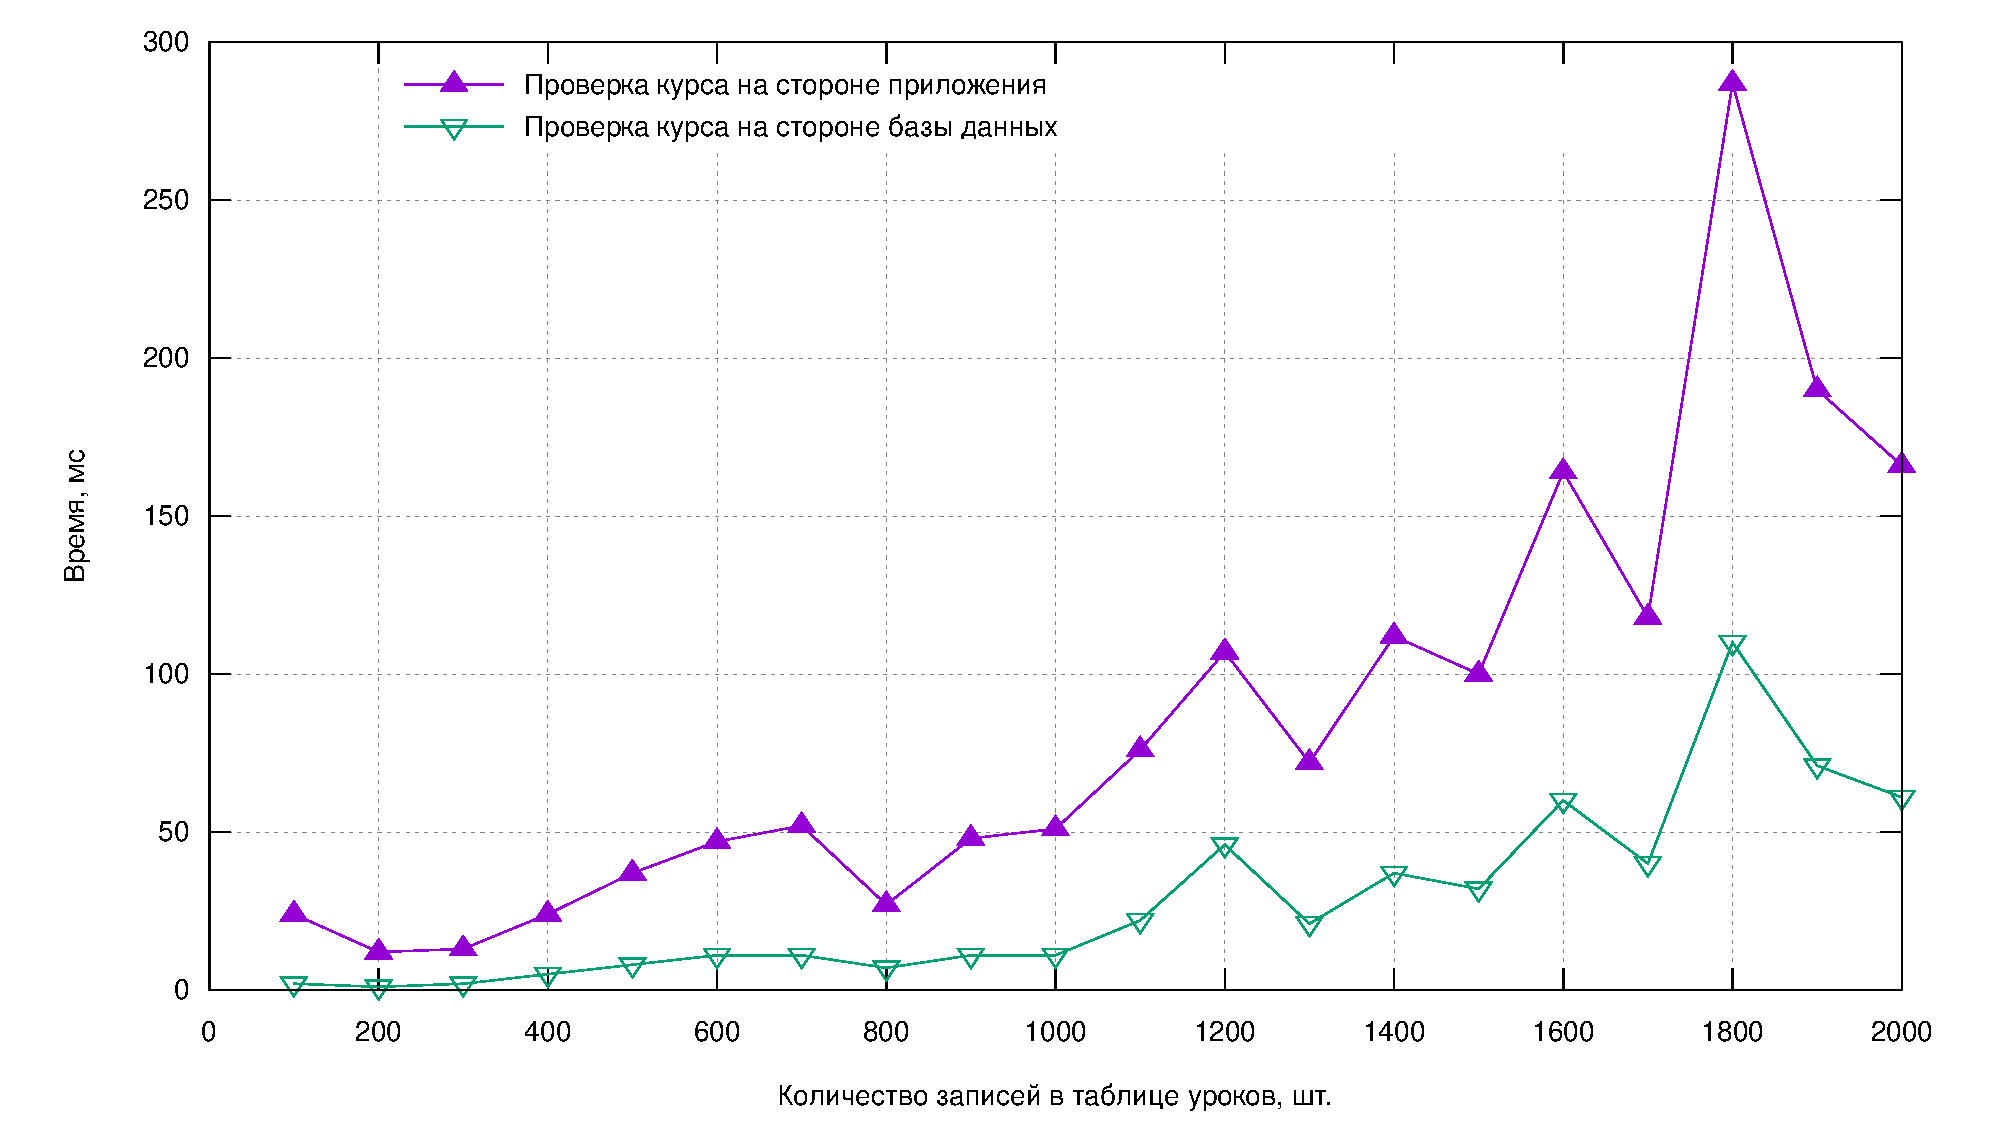
\includegraphics[height=0.35\textheight]{inc/img/plot2.pdf}
	\caption{График зависимости времени проверок целостности от количества уроков в курсе при диапазоне значений от 100 до 2000}
	\label{img:plot2}
\end{figure}

\section{Вывод из исследовательской части}

По результатом проведенного исследования видно, что проверки целостности курса на стороне приложения в 2-2.5 раза медленнее, чем проверки на уровне базы данных, с помощью триггера. При этом время выполнения проверок зависит линейно от количества записей в таблице уроков, поскольку целостность курса зависит от его наполнения уроками и требованиями, описанными ранее. 
